% Created 2020-08-17 Mon 13:40
% Intended LaTeX compiler: pdflatex
\documentclass[11pt]{article}
\usepackage[utf8]{inputenc}
\usepackage[T1]{fontenc}
\usepackage{graphicx}
\usepackage{grffile}
\usepackage{longtable}
\usepackage{wrapfig}
\usepackage{rotating}
\usepackage[normalem]{ulem}
\usepackage{amsmath}
\usepackage{textcomp}
\usepackage{amssymb}
\usepackage{capt-of}
\usepackage{hyperref}
\usepackage{minted}
\usepackage{../resources/referencing}
\addbibresource{../resources/references.bib}
\author{Ryan Greenup}
\date{\today}
\title{Relationship of Model Parameters and Solution Stability in the Power Walk Page Rank Method.}
\hypersetup{
 pdfauthor={Ryan Greenup},
 pdftitle={Relationship of Model Parameters and Solution Stability in the Power Walk Page Rank Method.},
 pdfkeywords={},
 pdfsubject={},
 pdfcreator={Emacs 27.1 (Org mode 9.4)}, 
 pdflang={English}}
\begin{document}

\maketitle
\tableofcontents

Ok. The discovery project is meant to be more of a data analysis project, so say
that you will be investigating the relationship between the second eigenvalue
and the model and graph parameters.

\section{{\bfseries\sffamily TODO} Introduction}
\label{sec:org19b18a9}
\begin{quote}
Your title should give a clear indication of your proposed research approach or
key question
\end{quote}

Much information is interconnected, \cite{teamSparseMatrixOperations}


another test reference \cite{kamvarAdaptiveMethodsComputation2004}

\section{{\bfseries\sffamily TODO} Background and Rationale}
\label{sec:orgf7c13c7}
\subsection{Background of issue and proposed research}
\label{sec:org5d62ccf}
\subsection{Indentify discipline}
\label{sec:org7f8213d}
\subsection{Summary of Developments in the field}
\label{sec:org34dce0a}
\section{{\bfseries\sffamily TODO} Literature Review}
\label{sec:org7c22388}
\subsection{Introduction}
\label{sec:org5b837e8}
\subsection{Body}
\label{sec:org2320536}
Structure the literature in a logical way
\subsubsection{Different Sources}
\label{sec:org9ba07d1}

\section{{\bfseries\sffamily TODO} Research Question}
\label{sec:org924ea90}
You should formulate these clearly, giving an explanation as to what problems
and issues are to be explored and why they are worth exploring* TODO Research
Methodology

\section{Research Methodology}
\label{sec:orgf061ffb}

\subsection{Theoretical Resources to be drawn on}
\label{sec:orgbe2f941}
\subsection{Research Approach}
\label{sec:orge8d8375}
\subsection{Advantages and disadvantages}
\label{sec:orgb258c2d}
\section{Plan of work}
\label{sec:org8288834}
\begin{itemize}
\item Regular consultations
\end{itemize}

\section{Notes}
\label{sec:org843f175}

\subsection{Question}
\label{sec:org2c91cae}

\emph{Can we determine the second eigenvalue from the method parameters? For
PageRank, the second eigenvalue is equal to the smoothing parameter \(\alpha\)}

\begin{quote}
Yes. An open question for the Power Walk method is, can we determine the second
eigenvalue from the method parameters? For PageRank, the second eigenvalue is
equal to the smoothing parameter \(\alpha\). The second eigenvalue determines how
long the algorithm takes to converge and how stable the solution is. To begin,
implement the method for computing PageRank and then the Power Walk. It can all
be done using sparse matrices, so it only requires a fraction of the memory and
is each iteration is quick.
\end{quote}

\subsection{Working}
\label{sec:orgf55dfe5}

Take the exemplar Graph from Figure 1:


\begin{listing}[htbp]
\begin{minted}[]{plantuml}
# #+begin_src javascript :exports code
@startdot
strict digraph graphName {
concentrate=true
fillcolor=green
color=blue
style="filled, rounded"
 A [shape=box, fillcolor="#a31621", style="rounded, filled"]

 edge [
    arrowhead="none"
  ];

 node[
    fontname="Fira Code",
    shape="square",
    fixedsize=false,
    style=rounded
  ];


# A -> B [dir="both"]
A -> B
B [shape=box, fillcolor="#bfdbf7", style="rounded, filled"]
B -> A
C [shape=box, fillcolor="#eaf4d3", style="rounded, filled"]
C -> D
D [shape=box, fillcolor="#0f5257", style="rounded, filled"]
D -> C
}
@enddot
\end{minted}
\caption{\label{DotLib}Code to Generate DOT Graph}
\end{listing}

\begin{center}
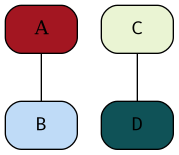
\includegraphics[width=.9\linewidth]{./Media/Example.png}
\end{center}



$$\begin{aligned} \Gamma = I - n D^{- 1}_B \\ \end{aligned}$$

Where we have the following:

\$\$\begin{aligned}
    \(\beta\) \&= 10 \\
    B \&= \(\beta\)\textsuperscript{A} \\
    A \&=
    \begin{bmatrix}
0& 1& 0& 0 \\
1& 0& 0& 0 \\
0& 0& 0& 1 \\
0& 0& 1& 0
    \end{bmatrix} \\
     \implies
    B &= \begin{bmatrix}
     10 & 1 & 1 & 1 \\
     1 & 10 & 1 & 1 \\
     1 & 1 & 10 & 1 \\
     1 & 1 & 1 & 10 \\
     \end{bmatrix}  \\
     \text{$D_B$ is a diagonal matrix of the column sums:}\\
     D &= \begin{bmatrix}
     13 & 0 & 0 & 0 \\
     0 & 13 & 0 & 0 \\
     0 & 0 & 13 & 0 \\
     0 & 0 & 0 & 13
     \end{bmatrix}  \\
     \text{Hence the Inverse is:}\\
     D_B^{-1}&= \frac{I}{13}\\
     \text{Putting it all together:}\\
     \Gamma &=  I - n D^{- 1}_B \\
     &= I - \frac{4 \cdot I}{13} \\
     &= \frac{9}{13} \cdot  I \\
     &= \begin{bmatrix}
         \frac{9}{13} & 0 & 0 & 0 \\
         0 & \frac{9}{13} & 0 & 0 \\
         0 & 0 & \frac{9}{13} & 0 \\
         0 & 0 & 0 &  \frac{9}{13}
     \end{bmatrix}  \\
     & \approx \begin{bmatrix}
         0.6923 & 0 & 0 & 0 \\
         0 & 0.6923 & 0 & 0 \\
         0 & 0 & 0.6923 & 0 \\
         0 & 0 & 0 & 0.6923
     \end{bmatrix}



\end{aligned}\$\$
\end{document}
